\chapter{Experiments} \label{chapter:experiments}

The following section describes the setups of the experiments conducted with the neural network presented in Chapter \ref{chapter:semi_automatic}. Due to the lack of existing annotated medical data the focus of the experiments is to ascertain a network design and mode of operation that compensate this as best as possible. First, we test the different network architectures that were described in section \ref{section:network_variations} using the same parameters. We then choose the best architecture for further experiments, in which we evaluate the two different training schemes introduced in section \ref{section:modes_of_operation}: training from scratch and incremental training.

\section{Terminology}

\noindent\textbf{Hyper-Parameter.} \textit{Hyper-parameters} are the tunable parameters of a network. The number and kind of parameters varies with the used type of network architecture, optimizer, etc.

\section{Datasets}

\begin{figure}[!tbp]
	\centering
	\begin{subfigure}[t]{0.47\textwidth}
		\centering
    	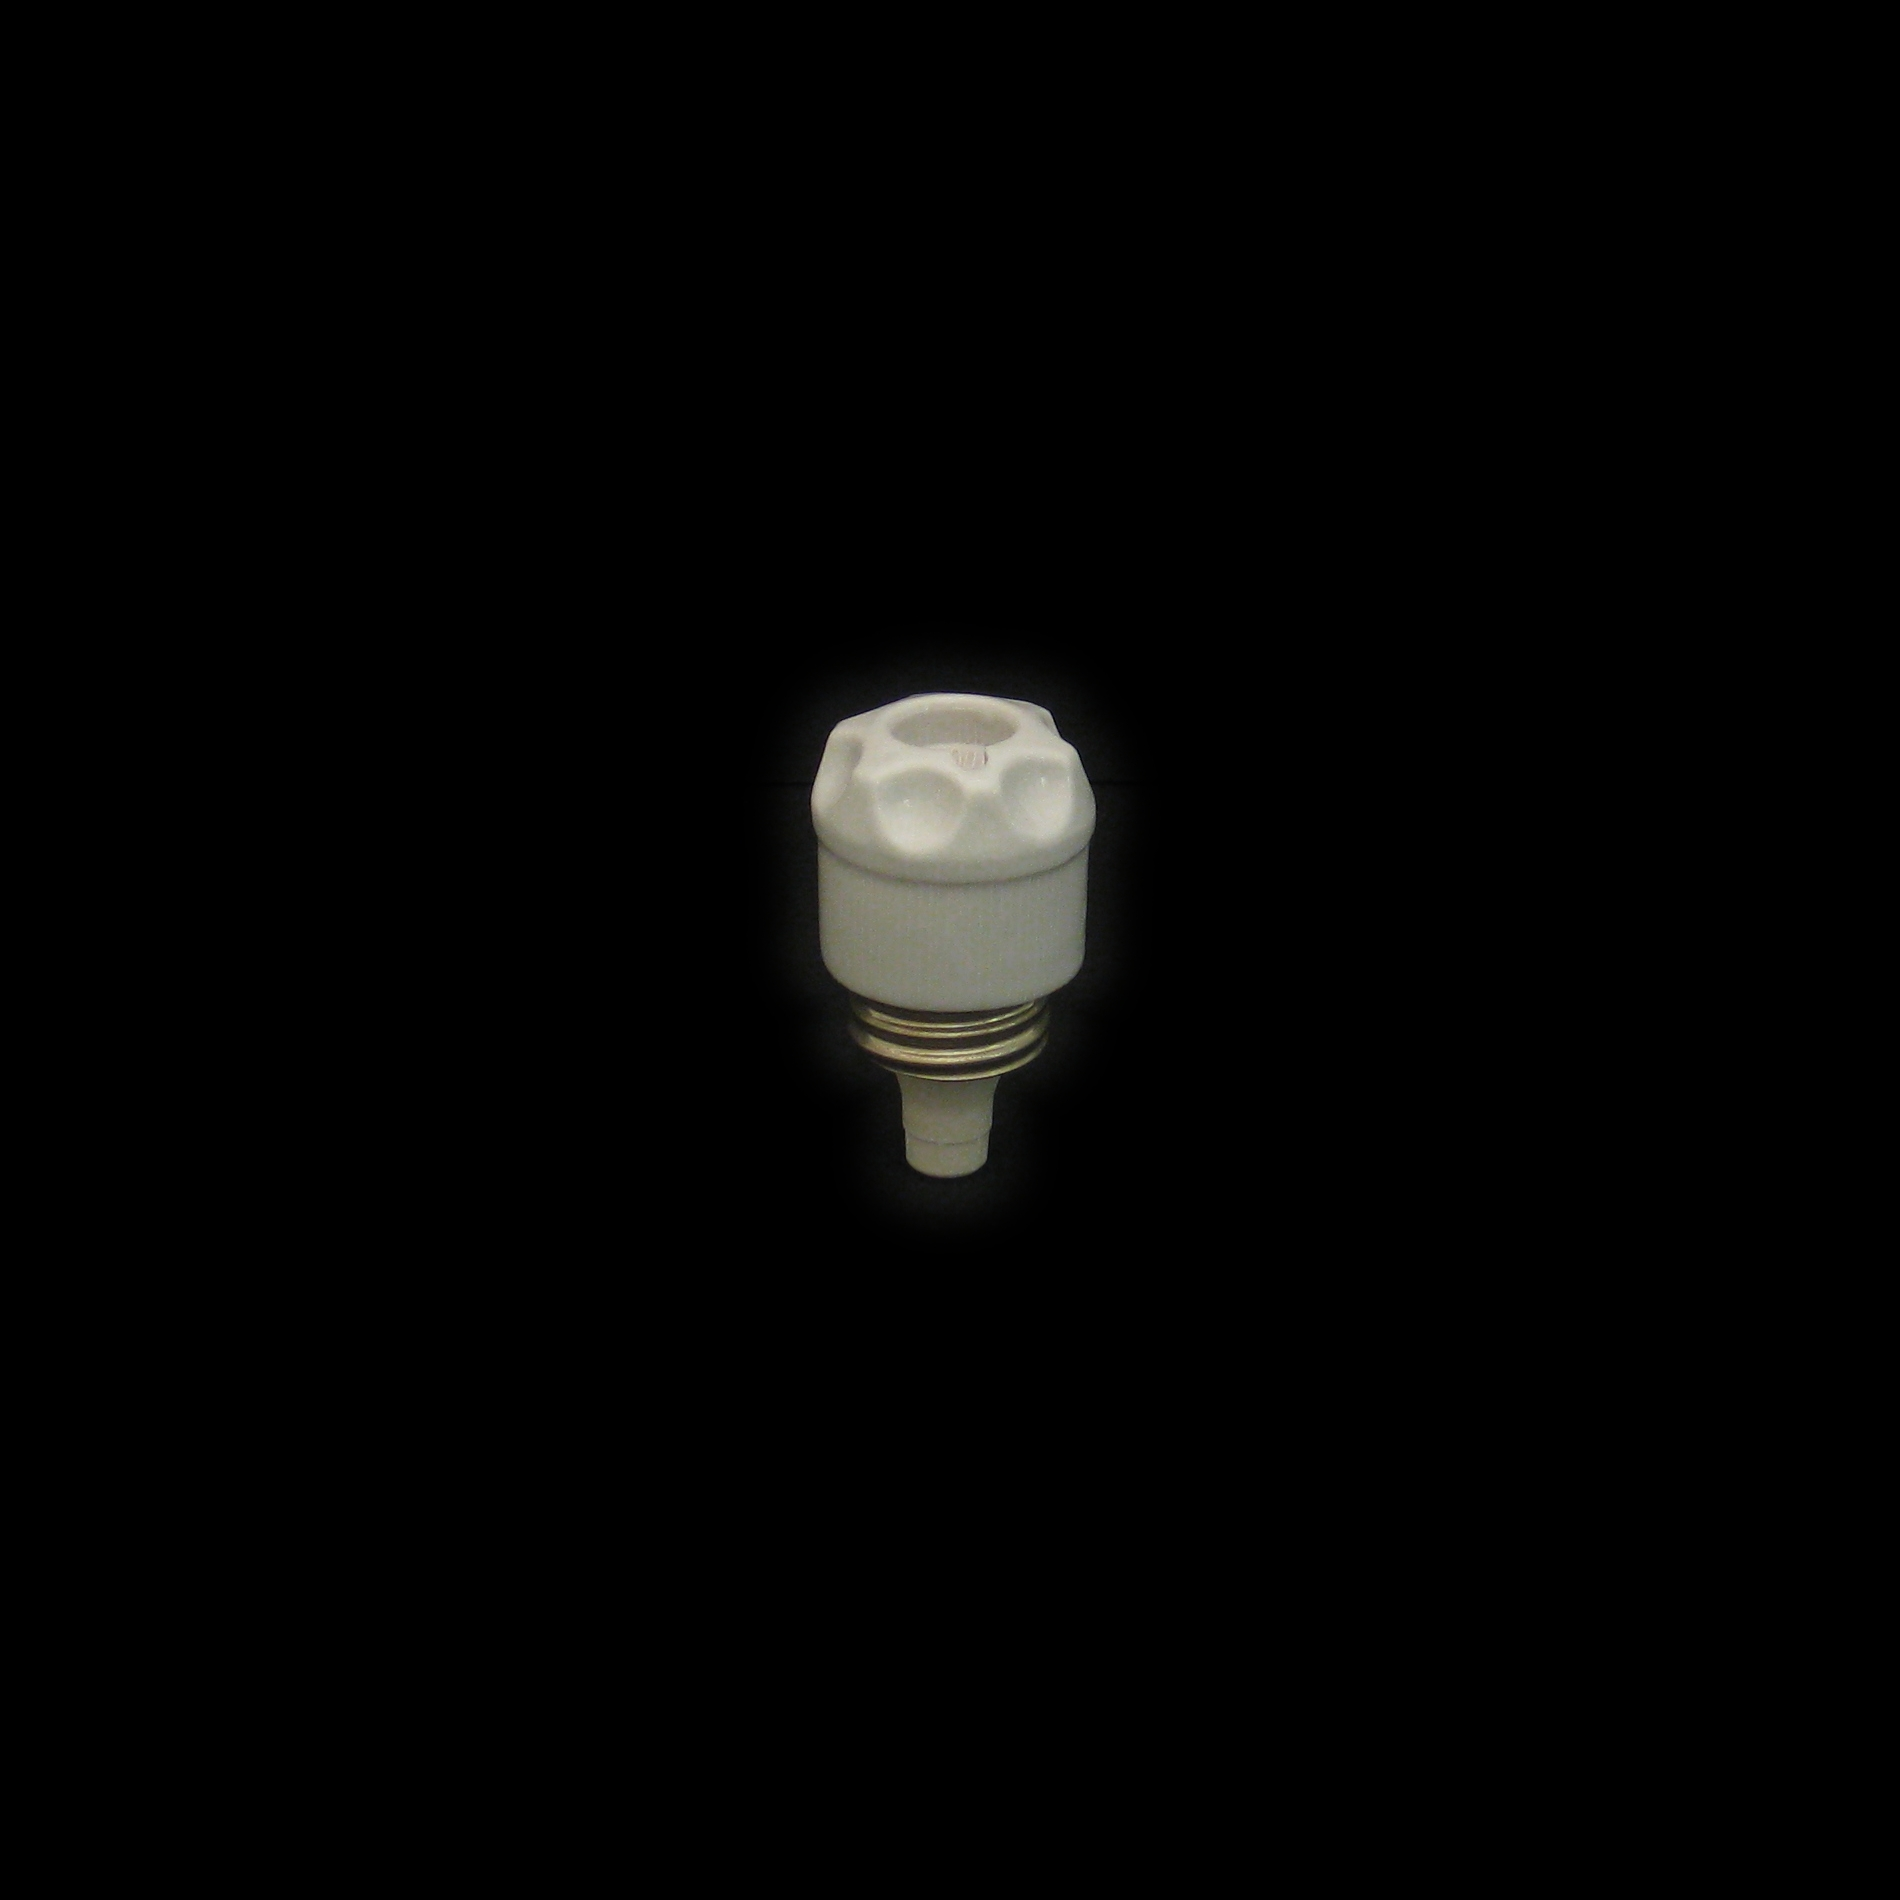
\includegraphics[width=0.6\linewidth]{tless_example_train}
    	\caption{An example frame from the training dataset of T-Less.}
    	\label{fig:tless_example_train}
	\end{subfigure}
	\hfill
	\begin{subfigure}[t]{0.47\textwidth}
		\centering
    	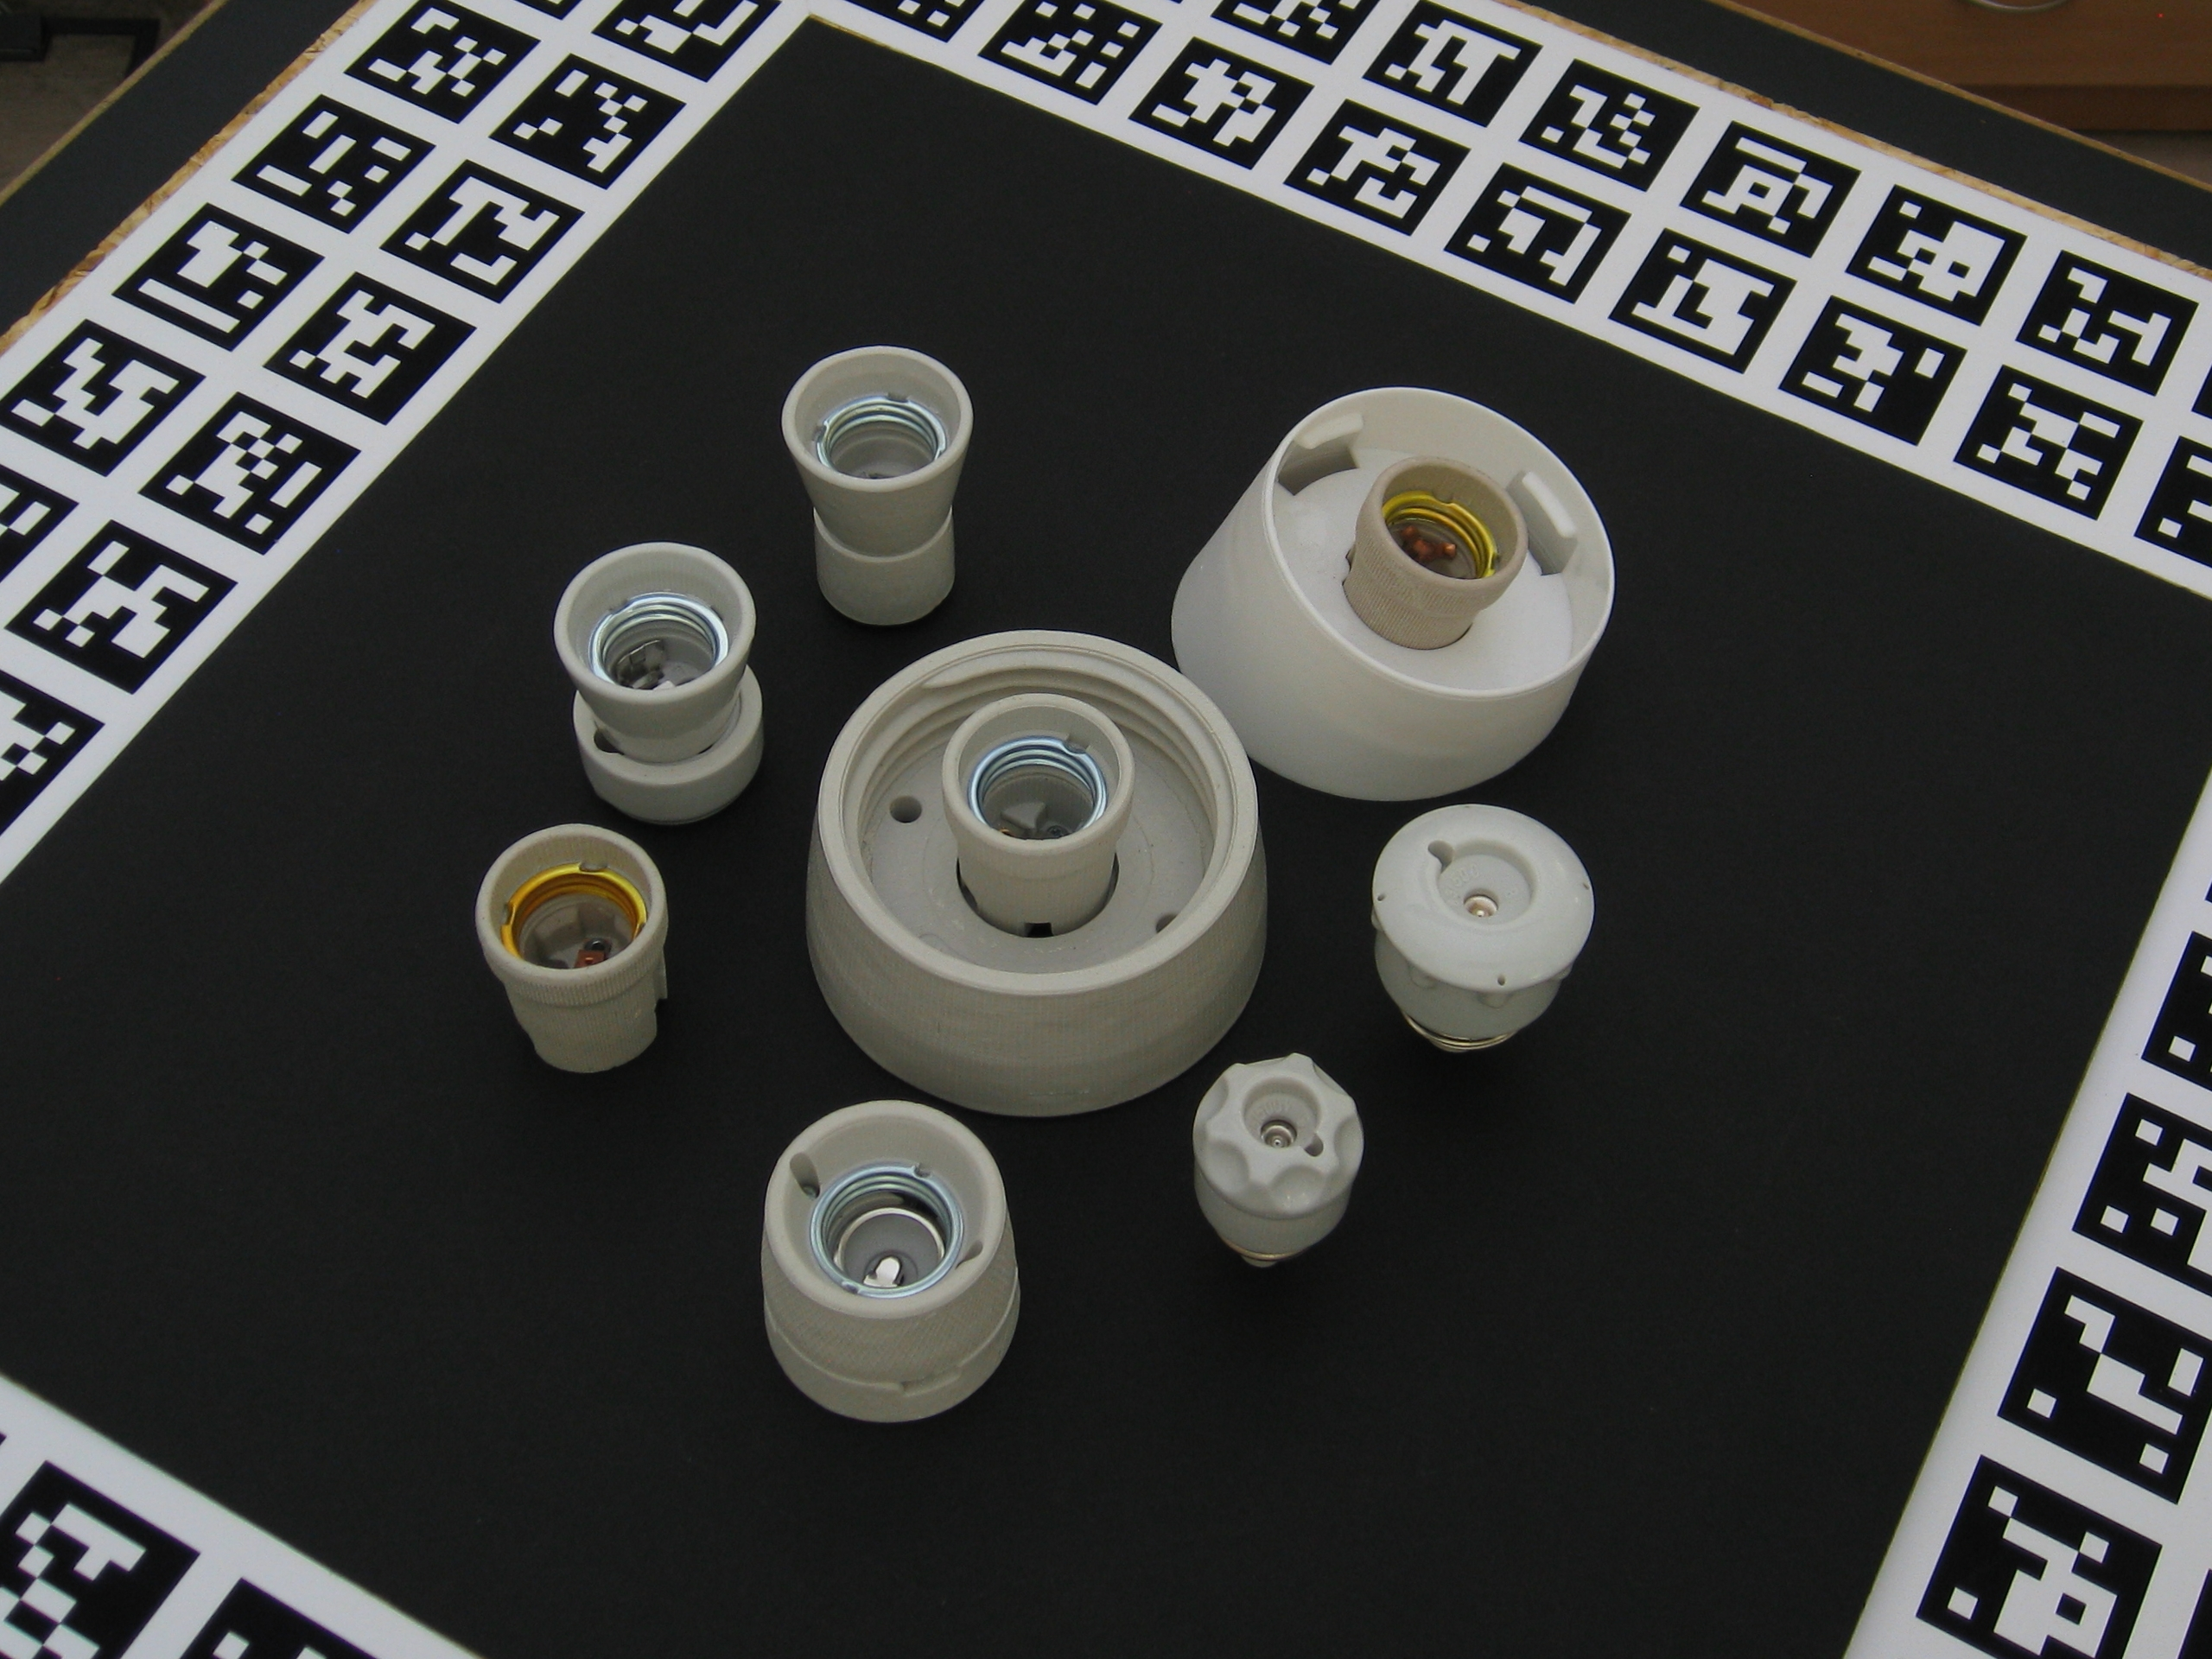
\includegraphics[width=0.7\linewidth]{tless_example_test}
    	\caption{An example frame from the test dataset of T-Less.}
    	\label{fig:tless_example_test}
	\end{subfigure}
	\caption{Example frames from the T-Less dataset \cite{tless}.}
	\label{fig:tless_examples}
\end{figure}

The initial intention to completely annotate the medical images provided at the beginning of the project turned out to be not feasible (see Chapter \ref{chapter:manual_annotation}). Instead, we chose the T-Less dataset to conduct the experiments with. Its objects are mostly texture-less  and of rather small size making them similar to surgical tools. Next to many human pose estimation datasets, there exist some datasets of objects too, like \cite{next_view_dataset}, \cite{pracsys_dataset} and \cite{rigid_body_dataset}. But the objects of T-Less resemble surgical tools more than the objects of those datasets.

The T-Less dataset was released in 2017 by Hoda\v{n} et al. \cite{tless}. It contains the object models of 30 industry-relevant real world objects. Two versions exist: one mesh of the object that was manually reconstructed using CAD software and one that was produced from RGB-D images. The 3D coordinates of the objects reflect their size in millimeters. For example, the minimum and maximum of any component of the coordinates of object model 01 are about -30 and 30. This means that the model is about 60 mm or 6 cm long. The objects were captured using a Primsense CARMINE 1.09, a Microsoft Kinect v2 and a Canon IXUS 950 IS. We used the photos of the Canon camera due to their quality and we do not need depth information, which is also provided by the CARMINE sensor and the Kinect. There are 1296 images of each object in the training set of the dataset, sampled in 10 degree steps in elevation and 5 degree azimuth. 20 test scenes, consisting of 504 images each, exist as well. Those are photographs of cluttered scenes of different complexity, with sometimes more than 15 objects visible. All training and test images are annotated with the ground-truth poses of the visible objects. The authors also provided a tool set to render the objects at a given pose, etc. Fig. \ref{fig:tless_example_train} shows an example frame from the training set and fig. \ref{fig:tless_example_test} an example frame from the test set. The training images of the other objects look similar to the one shown. The dataset provides depth images, as well, but this is irrelevant to our setting.

\section{Data Preparation}

The \textit{T-Less} dataset does neither provide 3D object coordinates nor segmentation masks. This is the reason why we rendered both ourselves. The script is part of the network package. Because the 16-bit TIFF object coordinate ground-truth files used up too much disk space when in original size they were cropped to the relevant area by determining the smallest box around the segmentation pixels. The images and segmentation masks were cropped to the same area and the camera matrices adjusted accordingly. We used 16-bit TIFF files instead of 32-bit because we deemed the accuracy of 16-bit enough.

\section{Metric}

We developed a set of evaluation metrics to capture different aspects of the prediction quality of a network. We assumed that multiple metrics provide better insights of the strengths and weaknesses of an architecture. To this end, we provide functionality that directly assesses the quality of the predicted object coordinates and also functionality that provides details on the accuracy of the resulting recovered pose.

The \textit{Object Coordinate Error} $e_{\text{coord}}$ computes the euclidean distances between the predicted and ground-truth object coordinates
\begin{align*}
e_{\text{coord}} = \frac{1}{|S_O|} \sum\limits_{(i, j)} \sqrt{(g_{ij1} - p_{ij1})^2 +(g_{ij2} - p_{ij2})^2 + (g_{ij3} - p_{ij3})^2}
\end{align*}
where $(i, j)$ are all 2D locations belonging to the object model $O$ according to the segmentation mask. $|S_O|$ denotes the cardinality of the set of these locations. $g_{ijk}$ and $p_{ijk}$ are the $k$-th components of the object coordinate at $(i, j)$ in the ground-truth and predicted object coordinates image, respectively.

The number of \textit{Inliers} $n_{\text{inlier}}$ captures the number of object coordinates whose euclidean distance to the ground-truth object coordinate is below a threshold:
\begin{align*}
e_{\text{inlier}} = \left\rvert\left\lbrace(i,j) \ \bigg| \ \sqrt{(g_{ij1} - p_{ij1})^2 +(g_{ij2} - p_{ij2})^2 + (g_{ij3} - p_{ij3})^2} \leq \sigma_{\text{thresh}}\right\rbrace \right\rvert
\end{align*}
where $\sigma_{\text{thresh}}$ is the chosen threshold and $(i,j)$ are again all locations belonging to the object model. We set the threshold to 2.

Both $e_{\text{coord}}$ and $n_{\text{inlier}}$ assess the accuracy of the predicted object coordinates. The metrics described next provide a measure of the quality of the recovered pose.

The \textit{Distance Error} $e_{\text{dist}}$ is the euclidean distance between the ground-truth position of the object and the position computed by \ac{ransac} by solving the \ac{pnp} problem. $e_{\text{dist}}$ is computed as
\begin{align*}
e_{\text{dist}} = \sqrt{(t_{g1} - t_{p1})^2 +(t_{g2} - t_{p2})^2 + (t_{g3} - t_{p3})^2}
\end{align*}
where $t_{gk}$ denotes the $k$-th component of the ground-truth translation vector, and $t_{pk}$ the $k$-th component of the translation vector recovered from the coordinate predictions.

The \textit{Angle Error} $e_{\text{angle}}$ is the rotational error in degrees between the ground-truth and calculated rotation matrix
\begin{align*}
e_{\text{angle}} = \frac{cos^{-1}(\frac{\Tr(R_g^TR_p) - 1}{2}) \cdot 180\degree}{\pi}
\end{align*}
where $R_g$ and $R_p$ denote the ground-truth and predicted rotation matrix, respectively and $Tr()$ denotes the trace of a matrix.

%TODO check if still actually used in the final version of the report

Finally, we also implemented the metric presented by Hinterstoisser \etal in \cite{hinterstoisser2}, which computes the average distance between each vertex of the object model with the ground-truth and recovered pose applied to it. This metric $e_{\text{pose}}$ is defined in the following way
\begin{align*}
e_{\text{pose}} = \frac{1}{|M|} \sum\limits_{X \in M}||(\bar{R}X + \bar{t}) - (RX + t)||
\end{align*}
for the set of points $M$ of an object model $O$. $\bar{R}$ and $\bar{t}$ denote the rotation matrix and translation vector of the ground-truth pose $\bar{P}$, while $R$ and $t$ are the respective components of the recovered pose.

\section{Training Experiments}

This section describes the configuration of the different training experiments. First, we compare the SGD and Adam optimizer in \ref{subsection:optimizers}. Then we evaluate the different architectures against each other in \ref{subsection:architectures}. Finally, asses the two training strategies training from scratch and incremental training in \ref{subsection:experiments_online_learning}. We conducted all experiments on the object model $01$ of the T-Less dataset. The image dimension was set to 500 pixels (for width and height), which is larger than the largest area covering an object in any image. All experiments were run using the training data of the object model $01$. For some experiments, we used only a subset of the available images (see Sections \ref{subsection:experiments_online_learning} and \ref{subsection:experiments_active_learning}) but we always split the data into 70\% training images and 30\% validation images while assigning the images to a set at random. If not stated otherwise, we used the same training and validation set throughout the experiments. The axis labeled \textit{epochs} in loss graphs denotes the number of epochs the training was run for. Each epoch consisted of 1000 iterations in every experiment.

\begin{table}[]
\centering
\begin{tabular}{|l||lllll|}
\hline
Run                                                     & 1     & 2      & 3       & 4        & 5         \\ \hline \hline
\rowcolor{Gray}
Epochs                                                  & 30    & 45     & 55      & 65       & 70        \\
\begin{tabular}[c]{@{}l@{}}Learning\\ Rate\end{tabular} & 0.001 & 0.0001 & 0.00001 & 0.000001 & 0.0000001 \\  \hline
\end{tabular}
\caption{The configuration of the SGD optimizer used in the experiment to compare SGD and Adam.}\label{table:experiments_optimizers_sgd}
\end{table}

\subsection{Optimizers} \label{subsection:optimizers}  

\begin{figure}[!tbp]
	\begin{subfigure}[t]{0.4\textwidth}
			\begin{tikzpicture}[scale=0.95]
  				\begin{axis}[cycle list name=tb, 
                 grid=both,
                 grid style={solid,gray!30!white},
                 axis lines=middle,
    			 xmin = 0,
    			 xmax = 60,
    			 ymin = 0,
    			 ymax = 9,
                 xlabel={epoch},
                 ylabel={loss},
                 x label style={at={(axis description cs:0.5,-0.1)},anchor=north},
                 y label style={at={(axis description cs:-0.1,.5)},rotate=90,anchor=south},]
      			\addplot[smooth,tb_color_1] table [x=Step, y=Value, col sep=comma] {experiments/model1/exp1_adam_l1/train_loss.csv};
      			\addplot[smooth,tb_color_2] table [x=Step, y=Value, col sep=comma] {experiments/model1/exp1_sgd/train_loss.csv};
      			\addlegendentry{Adam}
				\addlegendentry{SGD}
    			\end{axis}
			\end{tikzpicture}
		\caption{Training losses.}
	\end{subfigure}
	\hspace{15mm}
	\begin{subfigure}[t]{0.4\textwidth}
			\begin{tikzpicture}[scale=0.95]
  				\begin{axis}[cycle list name=tb, 
                 grid=both,
                 grid style={solid,gray!30!white},
                 axis lines=middle,
    			 xmin = 0,
    			 xmax = 60,
    			 ymin = 0,
    			 ymax = 9,
                 xlabel={epoch},
                 ylabel={loss},
                 x label style={at={(axis description cs:0.5,-0.1)},anchor=north},
                 y label style={at={(axis description cs:-0.1,.5)},rotate=90,anchor=south},]
      			\addplot[smooth,tb_color_1] table [x=Step, y=Value, col sep=comma] {experiments/model1/exp1_adam_l1/val_loss.csv};
      			\addplot[smooth,tb_color_2] table [x=Step, y=Value, col sep=comma] {experiments/model1/exp1_sgd/val_loss.csv};
      			\addlegendentry{Adam}
				\addlegendentry{SGD}
    			\end{axis}
			\end{tikzpicture}
		\caption{Validation losses.}
	\end{subfigure}
	\caption{Training and validation losses of Adam and SGD used to train architecture 1. The plot is cropped on the $y$-axis to enhance the differences.}
	\label{fig:experiments_adam_sgd_loss}
\end{figure} 

To obtain the best optimizer for further experiments, we compared SGD and Adam using the first architecture we constructed. This architecture consists of 23 layers and has a receptive field-size of 99. The hyper-parameters $\beta_1$ and $\beta_2$ of the Adam optimizer were left at the default values set by Keras, which are $0.9$ and $0.999$, respectively. The more complex configuration of the SGD optimizer is given in Table \ref{table:experiments_optimizers_sgd}. Fig. \ref{fig:experiments_adam_sgd_loss} shows the loss of both experiments during training. The SGD optimizer profits from the reduction of the learning rate around step 30, visible as the small step in the training loss. This could imply that further tuning of the training parameters of SGD could lead to better results than the displayed ones. But since the Adam optimizer does not need manual fine-tuning of its hyper-parameters and performs visibly better than SGD, we chose Adam as the optimizer for all following experiments. We based our conclusion that Adam is the superior optimizer for our network solely on the loss values. Since we trained the same network architecture twice and only varied the optimizers, better error rates mean better overall results.

\subsection{Loss Functions}

\begin{table}[]
\centering
\begin{tabular}{|l||llll|}
\hline 
 Loss  & $e_{\text{coord}}$ & $n_{\text{inlier}}$ & $e_{\text{angle}}$ & $e_{\text{dist}}$ \\ \hline \hline \rowcolor{Gray}
L1 & 0.3413                                                            & 1738    & 0.0281      & 4.5574         \\
L2 & 0.8188                                                            & 1617    & 0.1090      & 8.3138 \\ \hline   
\end{tabular}
\caption{The metrics of the experiments comparing the loss functions.}
\label{table:experiments_loss_functions}
\end{table}

%TODO maybe rewrite this "to prove our statment...." -> did we prove it???

To prove our statement that the L1 loss is more suitable than the L2 loss for our application, we conducted another training run using the L2 loss and compared it to the run using the L1 loss of the previous experiment. The loss function comparisons are depicted in \ref{fig:experiments_l1_l2_loss} but are omitted here, due to their limited comparability. To obtain the L2 loss, we removed taking the square root in computing the loss which naturally results in higher error rates. Table \ref{table:experiments_loss_functions} shows the metrics of the experiments with the different loss functions. The L1 loss offers clearly superior accuracy and is used in all further experiments.

\subsection{Architectures} \label{subsection:architectures}

%TODO WICHTIG: DRAUF EINGEHEN, WARUM ZB DAS NETZ MIT KLEINERER RECEPTIVE FIELD SIZE TIEFER SEIN MUSS ETC	

%TODO table of training parameters -> different batch sizes etc

%TODO keine Architektur 3, weil die einfach zu schlecht war -> keine gute Idee kleine receptive field size und flaches Netzwerk

%TODO We deemed the final performance to be more important when comparing architectures -> we compare the trainings on all images

\begin{figure}[!tbp]
	\begin{subfigure}[t]{0.4\textwidth}
			\begin{tikzpicture}[scale=0.95]
  				\begin{axis}[cycle list name=tb, 
                 grid=both,
                 grid style={solid,gray!30!white},
                 axis lines=middle,
                 xlabel={epoch},
    			 xmax = 70,
    			 ymax = 8,
                 ylabel={loss},
                 x label style={at={(axis description cs:0.5,-0.1)},anchor=north},
                 y label style={at={(axis description cs:-0.1,.5)},rotate=90,anchor=south},]
      			\addplot[smooth,tb_color_1] table [x=Step, y=Value, col sep=comma] {experiments/model1/exp1_adam_l1/train_loss.csv};
      			\addplot[smooth,tb_color_2] table [x=Step, y=Value, col sep=comma] {experiments/model2/train_loss.csv};
      			\addplot[smooth,tb_color_3] table [x=Step, y=Value, col sep=comma] {experiments/model3/train_loss.csv};
      			\addplot[smooth,tb_color_4] table [x=Step, y=Value, col sep=comma] {experiments/model4/train_loss.csv};
      			\addplot[smooth,tb_color_5] table [x=Step, y=Value, col sep=comma] {experiments/model5/exp1/train_loss.csv};
      			\addplot[smooth,tb_color_6] table [x=Step, y=Value, col sep=comma] {experiments/model6/train_loss.csv};
      			\addlegendentry{Architecture 1}
				\addlegendentry{Architecture 2}
				\addlegendentry{Architecture 3}
				\addlegendentry{Architecture 4}
				\addlegendentry{Architecture 5}
				\addlegendentry{Architecture 6}
    			\end{axis}
			\end{tikzpicture}
		\caption{Training losses.}
	\end{subfigure}
	\hspace{15mm}
	\begin{subfigure}[t]{0.4\textwidth}
			\begin{tikzpicture}[scale=0.95]
  				\begin{axis}[cycle list name=tb, 
                 grid=both,
                 grid style={solid,gray!30!white},
                 axis lines=middle,
                 xlabel={epoch},
    			 xmax = 70,
    			 ymax = 8,
                 ylabel={loss},
                 x label style={at={(axis description cs:0.5,-0.1)},anchor=north},
                 y label style={at={(axis description cs:-0.1,.5)},rotate=90,anchor=south},]
      			\addplot[smooth,tb_color_1] table [x=Step, y=Value, col sep=comma] {experiments/model1/exp1_adam_l1/val_loss.csv};
      			\addplot[smooth,tb_color_2] table [x=Step, y=Value, col sep=comma] {experiments/model2/val_loss.csv};
      			\addplot[smooth,tb_color_3] table [x=Step, y=Value, col sep=comma] {experiments/model3/val_loss.csv};
      			\addplot[smooth,tb_color_4] table [x=Step, y=Value, col sep=comma] {experiments/model4/val_loss.csv};
      			\addplot[smooth,tb_color_5] table [x=Step, y=Value, col sep=comma] {experiments/model5/exp1/val_loss.csv};
      			\addplot[smooth,tb_color_6] table [x=Step, y=Value, col sep=comma] {experiments/model6/val_loss.csv};
      			\addlegendentry{Architecture 1}
				\addlegendentry{Architecture 2}
				\addlegendentry{Architecture 3}
				\addlegendentry{Architecture 4}
				\addlegendentry{Architecture 5}
				\addlegendentry{Architecture 6}
    			\end{axis}
			\end{tikzpicture}
		\caption{Validation losses.}
	\end{subfigure}
	\caption{Training and validation losses of the different architectures. The $y$ axis is cropped to enhance the more delicate differences at the lower end. The validation losses of architectures 4 and 6 are too high to be displayed here.}
	\label{fig:experiments_architectures_loss}
\end{figure} 

The experiments run on the different architectures were all performed using the Adam optimizer with the parameters mentioned in Section \ref{subsection:optimizers} and the L1 loss. The major difference between the experiments is the architecture itself. The training process were run for a different number of iterations because some architectures converged earlier than others. The different losses are displayed in fig. \ref{fig:experiments_architectures_loss}.

\subsection{Online Learning} \label{subsection:experiments_online_learning}

%TODO Careful selection of images is important

%TODO  Check if number of images in plot is correct

%TODO mention that 25 images is easily achievable

%TODO mention how training and validation sets were created
      			
\begin{figure}[!tbp]
	\begin{subfigure}[t]{0.4\textwidth}
			\begin{tikzpicture}[scale=0.95]
  				\begin{axis}[cycle list name=tb, 
                 grid=both,
                 grid style={solid,gray!30!white},
                 axis lines=middle,
                 xlabel={epoch},
    			 xmax = 50,
                 ylabel={loss},
                 x label style={at={(axis description cs:0.5,-0.1)},anchor=north},
                 y label style={at={(axis description cs:-0.1,.5)},rotate=90,anchor=south},]
      			\addplot[smooth,tb_color_1] table [x=Step, y=Value, col sep=comma] {experiments/model1/exp1_adam_l1/train_loss.csv};
      			\addplot[smooth,tb_color_2] table [x=Step, y=Value, col sep=comma] {experiments/model1/exp2/train_loss.csv};
      			\addplot[smooth,tb_color_2] table [x=Step, y=Value, col sep=comma] {experiments/model1/exp3/train_loss.csv};
      			\addplot[smooth,tb_color_3] table [x=Step, y=Value, col sep=comma] {experiments/model1/exp4/train_loss.csv};
      			\addplot[smooth,tb_color_4] table [x=Step, y=Value, col sep=comma] {experiments/model1/exp5/train_loss.csv};
      			\addplot[smooth,tb_color_5] table [x=Step, y=Value, col sep=comma] {experiments/model1/exp6/train_loss.csv};
      			\addlegendentry{All}
      			\addlegendentry{500}
				\addlegendentry{250}
				\addlegendentry{100}
				\addlegendentry{50}
				\addlegendentry{25}
    			\end{axis}
			\end{tikzpicture}
		\caption{Training losses.}
	\end{subfigure}
	\hspace{15mm}
	\begin{subfigure}[t]{0.4\textwidth}
			\begin{tikzpicture}[scale=0.95]
  				\begin{axis}[cycle list name=tb, 
                 grid=both,
                 grid style={solid,gray!30!white},
                 axis lines=middle,
                 xlabel={epoch},
    			 xmax = 50,
                 ylabel={loss},
                 x label style={at={(axis description cs:0.5,-0.1)},anchor=north},
                 y label style={at={(axis description cs:-0.1,.5)},rotate=90,anchor=south},]
      			\addplot[smooth,tb_color_1] table [x=Step, y=Value, col sep=comma] {experiments/model1/exp1_adam_l1/val_loss.csv};
      			\addplot[smooth,tb_color_2] table [x=Step, y=Value, col sep=comma] {experiments/model1/exp2/val_loss.csv};
      			\addplot[smooth,tb_color_2] table [x=Step, y=Value, col sep=comma] {experiments/model1/exp3/val_loss.csv};
      			\addplot[smooth,tb_color_3] table [x=Step, y=Value, col sep=comma] {experiments/model1/exp4/val_loss.csv};
      			\addplot[smooth,tb_color_5] table [x=Step, y=Value, col sep=comma] {experiments/model1/exp5/val_loss.csv};
      			\addplot[smooth,tb_color_5] table [x=Step, y=Value, col sep=comma] {experiments/model1/exp6/val_loss.csv};
      			\addlegendentry{All}
      			\addlegendentry{500}
				\addlegendentry{250}
				\addlegendentry{100}
				\addlegendentry{50}
				\addlegendentry{25}
    			\end{axis}
			\end{tikzpicture}
		\caption{Validation losses.}
	\end{subfigure}
	\caption{Training and validation losses of the experiments of training architecture \textbf{1} from scratch but not with all images. The keys are the number of images used in training.}
	\label{fig:experiments_online_sratch_loss}
\end{figure} 

% Nochmal zusammenfassen scratch vs inkrementell

\subsection{Active Learning} \label{subsection:experiments_active_learning}

% Training on one side only -> provide metric results -> training on bad images -> new metrics

\subsection{Runtime Analysis}

This section analyses the inference runtimes of the different architectures. Deeper networks need longer to perform training and an inference run on an image, which is reflected by table ...

\subsection{Limitations}

% No challenge yet, difficult to tell how good network is -> no baseline!

% T-Less dataset contains only unoccluded images

% This way of comparing training procedures is owned to the timeframe of this work -> maybe L2 works better for model 5, etc., we generalize from one model to all others

% Create metric for images that the network produces bad predictions for, e.g. reprojection error for contradicting object coordinates, difference between segmentation mask rendered using the predicted pose and the ground-truth segmentation mask -> was not possible because we couldn't annotate images of the Endovis dataset

% Maybe training - validation ratio should be more like 90 - 10

% Difficult to say how the network would perform on the Endovis dataset -> we don't know if the networks with larger receptive field-size predict based on the letters
